\documentclass[Space_Shuttle_Vessel_Manual.tex]{subfiles} 
\begin{document}

\section{PAYLOADS}
\begin{multicols*}{2}
\label{sec:payloads}
\renewcommand{\cfttoctitlefont}{\bf}
\localtableofcontents
\noindent
\\
Like the real Space Shuttle, SSV allows the user to place payloads in the Payload Bay (PLB). This chapter explains how payloads (satellites, space station modules, small experiment canisters, etc) can be attached to the PLB. Details are also provided about the attachment needed for payloads to be grappled by the RMS.\\
In addition to basic payload information, this section contains data on how payloads can be used in SSV.

\end{multicols*}

\begin{multicols*}{2}
\subsection{Payload Types}
\noindent
SSV groups payloads into 5 categories, according to the location and way they are attached in the PLB: "Active", "Passive", "Bay Bridge", "Manipulator Position Mechanism (MPM)" and "Upper Stage".
\\
The first 2 groups of payloads represent the most common payloads. They are attached to the PLB with payload retention latches capable of holding the largest payloads the Space Shuttle can carry. "Active" payloads can be released and latched (e.g., LDEF), while "Passive" payloads remain in the PLB for the duration of the mission (e.g., Spacelab).
\\
The "Bay Bridge" payloads are mounted in place of the payload bay attachment bridges, on the PLB sill longerons or the keel. They are usually brackets for mounting small payloads (e.g. Get Away Special (GAS) Canisters).
\\
The Manipulator Position Mechanism (MPM) payloads attach to the MPM pedestals. The most common example of this type of payload is the Orbiter Boom Sensor System (OBSS).
\\
The Upper Stage payloads are detailed in section \ref{sec:upper-stages}.


\subsubsection{Active}
These payloads are connected to the PLB with active latches, allowing the payloads to be released and latched as needed. Bridges spanning the payload bay frames at the sill longeron and keel provide mounting locations for the latches, in predetermined locations at every 3.933 inches. These locations are identified by their PLID number.
A maximum of 5 "Active" payloads can be defined for a mission.
\\
Each payload can specify up to 12 latches (4 port, 4 starboard and 4 keel), although payloads usually use a 3-point (2 longeron, 1 keel) or 5-point (4 longeron, 1 keel) system.
One of these attachments is defined to be the "main" attachment, which corresponds to the vessel attachment point. The attachment should usually be placed at one of the keel latches, but it is permitted to be placed at one of the sill longeron latches. Each latch is wired to a latch control system to allow for its operation from controls on panel A6U.
\\
Sill longeron latches can be fitted with extended guides, for ease of deploy and latch operations.
\\
The location of the attachment point is the center of the latches. At the keel, that is Yo 0.0 and Zo+305.025 for bays 1-11, Zo+308.40 for bay 12. For attachments at the sill longeron, the location is Yo+/-93.925 and Zo+414.05. Each PLID is fixed at a longitudinal (Xo) position. The forward-most PLID is 154 at Xo+608.80, and the aft-most PLID is 330 at Xo+1303.00. A section of the 90-inch radius payload envelope, with the location of the available attachment locations is show in figure \ref{fig:payload_attachment}.
\\
The attachment direction and rotation vectors for a keel-attached payload are shown in figure \ref{fig:PLkeelattach}, and for longeron-attached payloads in figure \ref{fig:PLlongeronattach}.
\begin{figure}[H]
  \centering
  \captionsetup{justification=centering}
  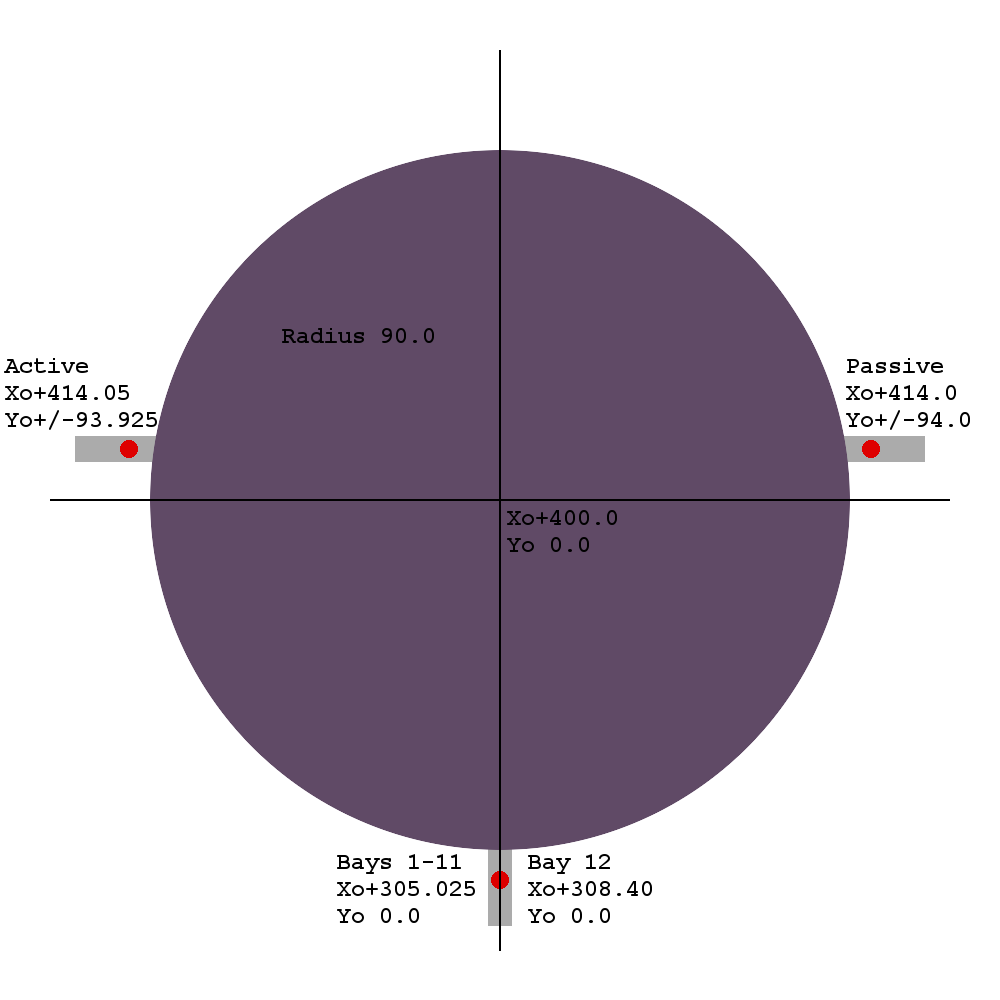
\includegraphics[width=0.99\hsize]{payload_attachment.png}
  \caption{Section of payload envelope with attachment locations}
  \label{fig:payload_attachment}
\end{figure}
\begin{figure}[H]
  \centering
  \captionsetup{justification=centering}
  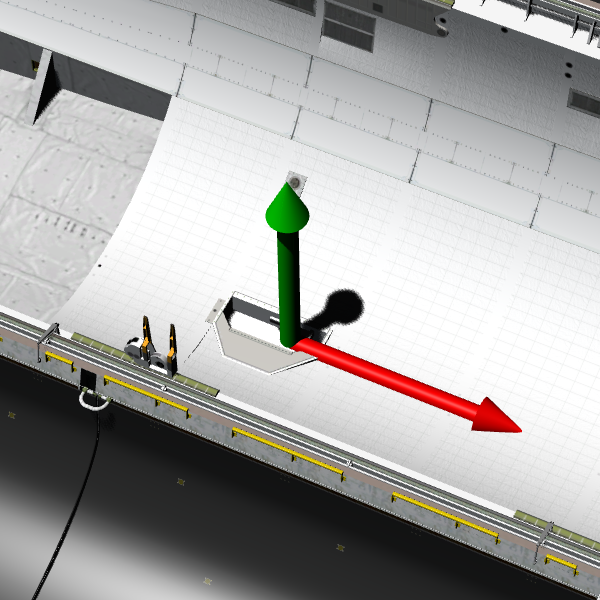
\includegraphics[width=0.99\hsize]{PLkeelattach.png}
  \caption{Active and Passive payload keel attachment direction (green) and rotation (red)}
  \label{fig:PLkeelattach}
\end{figure}
\begin{figure}[H]
  \centering
  \captionsetup{justification=centering}
  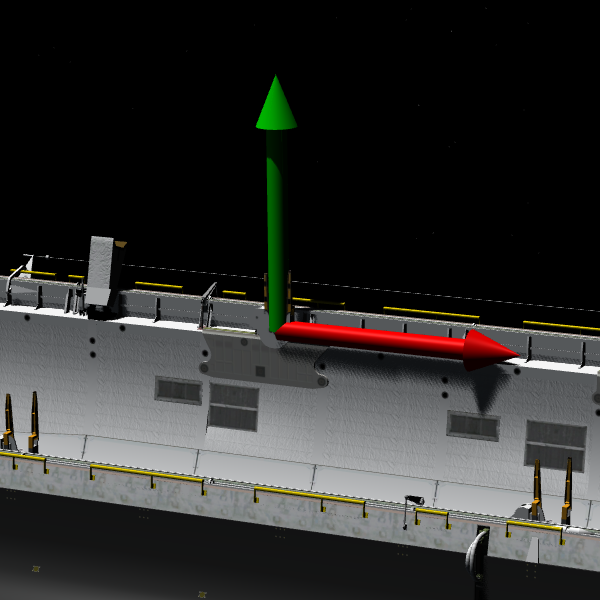
\includegraphics[width=0.99\hsize]{PLlongeronattach.png}
  \caption{Active and Passive payload longeron attachment direction (green) and rotation (red)}
  \label{fig:PLlongeronattach}
\end{figure}


\subsubsection{Passive}
If a payload doesn't need to be released in-flight, it is attached to the PLB with passive latches. Up to 5 "Passive" payloads can be defined.
\\
The attachment scheme is similar to the one used for the "Active" payloads, also with a similar 12 latch limit. The location of attachments defined at the keel is Yo 0.0 and Zo+305.025 for bays 1-11, Zo+308.40 for bay 12. If defined at the sill longeron, the location is Yo+/-94.0 and Zo+414.0. A section of the 90-inch radius payload envelope, with the location of the available attachment locations is show in figure \ref{fig:payload_attachment}.
\\
The attachment direction and rotation vectors for a keel-attached payload are shown in figure \ref{fig:PLkeelattach}, and for longeron-attached payloads in figure \ref{fig:PLlongeronattach}.


\subsubsection{Bay Bridge}
"Bay Bridge" payloads are mounted on the sill longeron and ring frame attachments, usually used for the payload bay attachment bridges, effectively replacing them. These payload attachments are not releasable in during the mission, and are usually used to attach mounting plates for other payloads (e.g. payload canisters). A combined total of 8 "Bay Bridge" payloads (port, starboard and keel) can be defined. All 13 bays are available for the sill longeron bridges, but only 12 bays (1 thru 12) for the keel bridge.
\\
The attachment point is defined at the center point between the 2 PLB ring frames bordering the bay at Zo+408.0 and Yo+/-94.0 for the sill longeron bridges, and Zo+306.0 and Yo 0.0 for the keel bridges. The Xo coordinates for the bay limits and the location of the attachment are listed in Table \ref{tab:BayCoordinates}


\begin{table}[H]
  \centering
  \begin{tabularx}{210pt}{c | >{\centering\arraybackslash}p{50pt} | >{\centering\arraybackslash}p{50pt} | >{\centering\arraybackslash}p{50pt}}
    \textbf{Bay} & \textbf{Forward ring frame} & \textbf{Attachment location} & \textbf{Aft\newline ring frame} \\
    \hline
    1 & 582.0 & 609.0 & 636.0 \\
    2 & 636.0 & 664.5 & 693.0 \\
    3 & 693.0 & 721.5 & 750.0 \\
    4 & 750.0 & 778.5 & 807.0 \\
    5 & 807.0 & 835.0 & 863.0 \\
    6 & 863.0 & 891.0 & 919.0 \\
    7 & 919.0 & 949.25 & 979.5 \\
    8 & 979.5 & 1009.75 & 1040.0 \\
    9 & 1040.0 & 1065.165 & 1090.33 \\
    10 & 1090.33 & 1115.5 & 1140.67 \\
    11 & 1140.67 & 1165.835 & 1191.0 \\
    12 & 1191.0 & 1220.0 & 1249.0 \\
    13 & 1249.0 & 1278.0 & 1307.0
  \end{tabularx}
  \caption{Bay Xo Coordinates}
  \label{tab:BayCoordinates}
\end{table}

\noindent
The attachment direction and rotation vectors for a longeron-attached payload are shown in figure \ref{fig:BBlongeronattach}, and for keel-attached payloads in figure \ref{fig:BBkeelattach}.
\begin{figure}[H]
  \centering
  \captionsetup{justification=centering}
  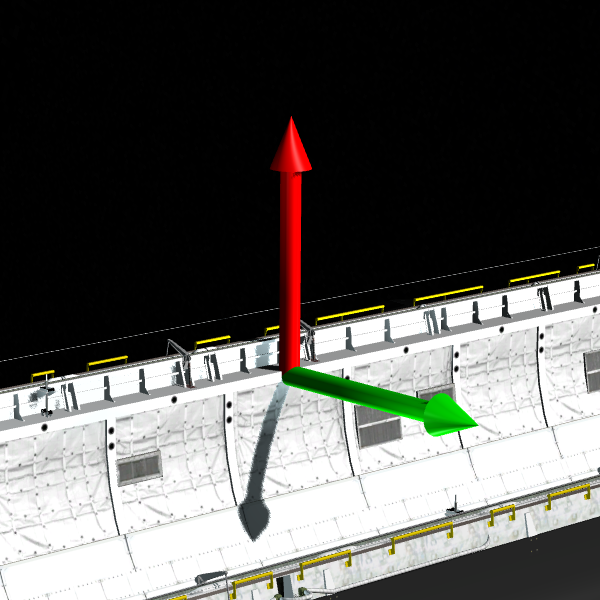
\includegraphics[width=0.99\hsize]{BBlongeronattach.png}
  \caption{Bay bridge payload longeron attachment direction (green) and rotation (red)}
  \label{fig:BBlongeronattach}
\end{figure}
\begin{figure}[H]
  \centering
  \captionsetup{justification=centering}
  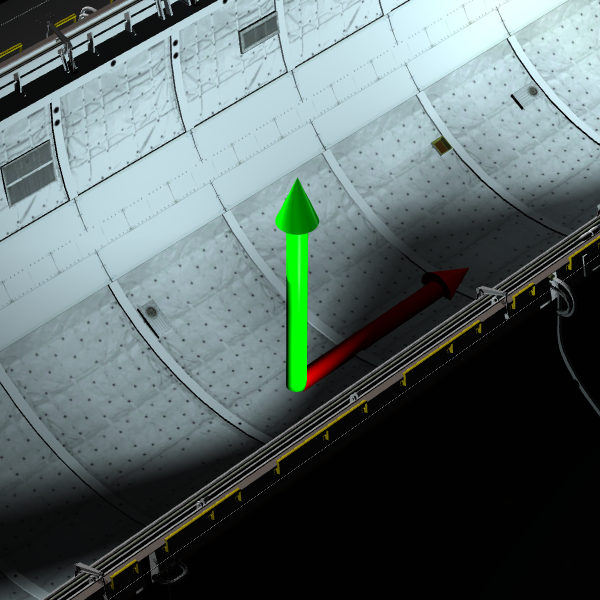
\includegraphics[width=0.99\hsize]{BBkeelattach.png}
  \caption{Bay bridge payload keel attachment direction (green) and rotation (red)}
  \label{fig:BBkeelattach}
\end{figure}


\subsubsection{MPM}
In addition to providing a mounting place for the RMS, the Manipulator Positioning Mechanism (MPM) pedestals can also be used for payload purposes (when the RMS is not used). These payloads can be latched and released from the 4 MPM pedestals with switches on panel A8A2.
The number of MPM pedestals needed for a payload, and the upper pedestal mesh, are configurable in the mission file (see \ref{sec:mission-configuration}). The OBSS is an example of a MPM payload. MPM upper pedestal meshes for the OBSS are provided in SSV.\\
The attachment point for these payloads is located inside one of the MPM pedestals, and the payloads must have its attachment in the strike-bar. The Xo location of the pedestals is listed in table \ref{tab:MPMCoordinates}.

\begin{table}[H]
  \centering
  \begin{tabularx}{125pt}{c | c}
    \textbf{Pedestal} & \textbf{Xo coordinate} \\
    \hline
    Shoulder & 679.5 \\
    Forward & 911.05 \\
    Mid & 1189.0 \\
    Aft & 1256.5
  \end{tabularx}
  \caption{MPM pedestal Xo Coordinates}
  \label{tab:MPMCoordinates}
\end{table}

\noindent
The attachment direction and rotation vectors for a payload are shown in figure \ref{fig:MPMPLattach}.
\begin{figure}[H]
  \centering
  \captionsetup{justification=centering}
  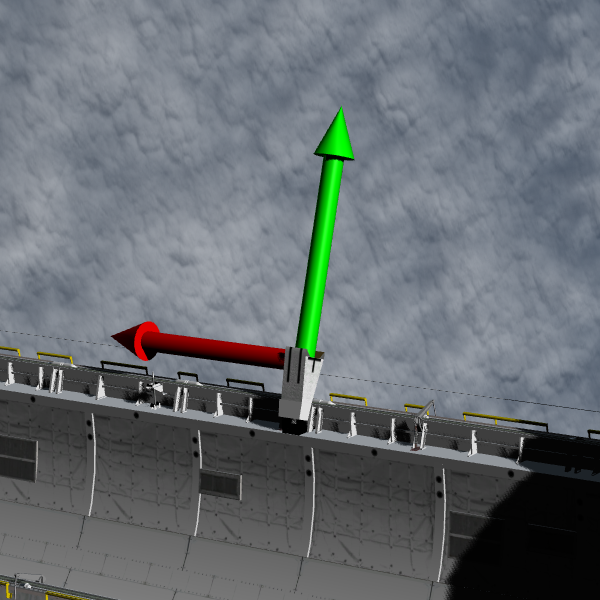
\includegraphics[width=0.99\hsize]{MPMPLattach.png}
  \caption{MPM payload attachment direction (green) and rotation (red)}
  \label{fig:MPMPLattach}
\end{figure}


\subsection{RMS}
For the RMS to grapple a payload, it much have an attachment with the ID "G". The attachment must be placed at the surface of the Grapple Fixture plate, centered in the cam/arm assembly.
\\
The attachment direction and rotation vectors for the RMS End Effector are shown in figure \ref{fig:RMSattach}.
\begin{figure}[H]
  \centering
  \captionsetup{justification=centering}
  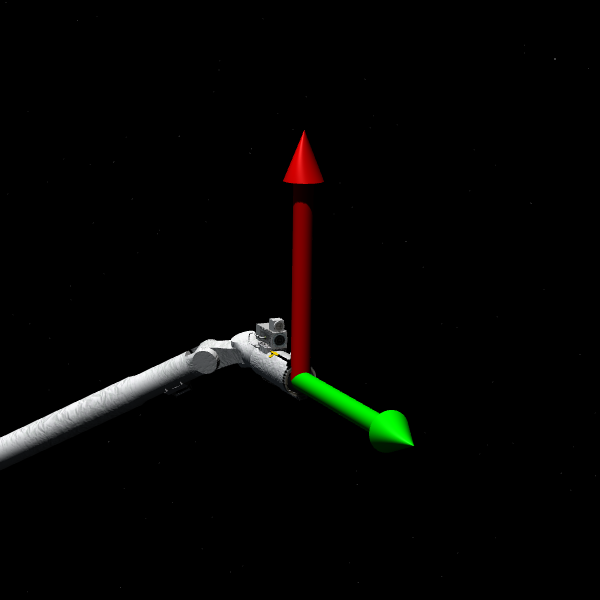
\includegraphics[width=0.99\hsize]{RMSattach.png}
  \caption{RMS payload attachment direction (green) and rotation (red)}
  \label{fig:RMSattach}
\end{figure}

\end{multicols*}
\end{document}